\section{Ramanujanovi grafi}
Koncept ramanujanovih grafov ima enostavno definicijo, vendar njen pomen ni očiten brez predhodne motivacije s sorodnimi definicijami in izreki. Te nam razjasnijo povezavo med lastnimi vrednostmi grafa, ki se pojavijo v definiciji Ramanujanovih grafov, ter povezljivostjo grafa.
\subsection{Cheegerjeva konstanta}
Kot v uvodnem primeru nas zanima koliko povezav moremo odstraniti, da graf ni več povezan.

Naj bo \(G=(V,E)\) povezan graf in \(S\subseteq V\) podmnožica vozlišč z \(0<\lvert S \rvert \leq \frac{\lvert V \rvert}{2}\). Z \(\partial S\subseteq E\) označimo množico povezav od \(S\) do komplementa vozlišč, \(\overline{S}\). Če iz grafa odstranimo \(\partial S\), potem se graf postane nepovezan.

Najbolj problematična so ozka grla grafa. To je majhna množica povezav, ki ločuje dva dela grafa z veliko vozlišči. Da je graf dobro povezan torej želimo, da ni ozkih grl in da je za velik \(\lvert S\rvert\) tudi velik \(\lvert \partial S\rvert \), oziroma da \(\frac{\lvert S\rvert}{\lvert \partial S\rvert}\) ni nikoli majhen.

% reword T?
\begin{definicija}[Cheegerjeva konstanta]
    Za graf \(G = (V,E)\) in njegova vozlišča \(T = \left\{S\subseteq V \mid 0<\lvert S \rvert \leq \frac{\lvert V \rvert}{2}\right\}\) definiramo Cheegerjevo konstanto kot
    \begin{align*}
        c(G) = \min_{S\in T} \frac{\lvert \partial S\rvert}{\lvert S\rvert}
    \end{align*}
\end{definicija}
Večji kot je \(c(G)\), manj ozkih grl ima graf \(G\).

\begin{primer}[Cikli]
    \hspace{0em}
    \begin{center}
        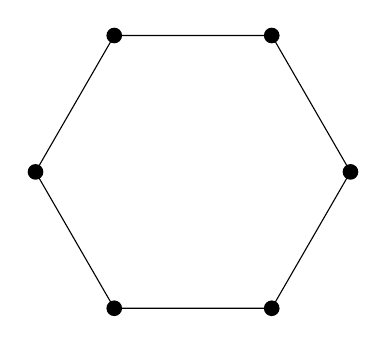
\begin{tikzpicture}
            % Defining the vertices of the cycle
            \foreach \x in {0,60,...,300} {
                    \node[circle, fill=black, inner sep=2pt] at (\x:2) {};
                }
            % Drawing the edges of the cycle
            \draw (0:2) -- (60:2) -- (120:2) -- (180:2) -- (240:2) -- (300:2) -- cycle;
        \end{tikzpicture}
    \end{center}

    Da minimiziramo \(\frac{\lvert \partial S\rvert}{\lvert S\rvert}\) lahko vzamemo sosednja vozlišča. Tako bo vedno \(\lvert \partial S\rvert = 2\), \(S\) pa povečamo do polovice cikla, kot omejuje definicija. Za cikel \(C_{2n}\) torej vzamemo \(\lvert S\rvert = n\), za \(C_{2n+1}\) pa prav tako \(\lvert S\rvert = n\).
    \begin{align*}
        c(C_n) = \frac{2}{\lfloor \frac n2\rfloor}
    \end{align*}
    Večji kot je \(n\), manjša je Cheegerjeva konstanta in graf je slabše povezan, saj rabimo odstraniti le dve povezavi da ločimo veliko vozlišč od preostanka.
\end{primer}
\begin{primer}[Polni grafi]
    \hspace{0em}
    \begin{center}
        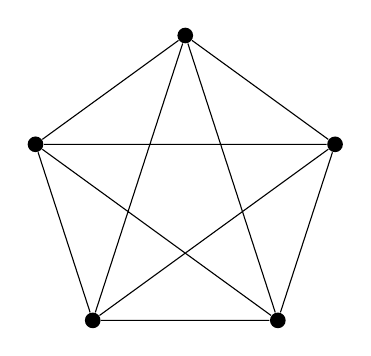
\begin{tikzpicture}
            \node[circle, fill=black, inner sep=2pt] (A) at (90:2) {};
            \node[circle, fill=black, inner sep=2pt] (B) at (162:2) {};
            \node[circle, fill=black, inner sep=2pt] (C) at (234:2) {};
            \node[circle, fill=black, inner sep=2pt] (D) at (306:2) {};
            \node[circle, fill=black, inner sep=2pt] (E) at (18:2) {};
            \draw (A) -- (B) -- (C) -- (D) -- (E) -- (A);
            \draw (A) -- (C) -- (E) -- (B) -- (D) -- (A);
        \end{tikzpicture}
    \end{center}
    Za graf \(K_n\) velja, da je \(\lvert \partial S\rvert = \lvert S\rvert \cdot (n - \lvert S\rvert)\). Torej je
    \begin{align*}
        c(K_n) = \min_{S} n-\lvert S\rvert
    \end{align*}
    minimum je dosežen pri \(\lvert S\rvert = \lfloor\frac n2\rfloor\) s poljubno izbiro vozlišč.
    \begin{align*}
        c(K_n) = \left\lceil \frac n2 \right\rceil
    \end{align*}
    Večji kot je \(n\), večja je Cheegerjeva konstanta in graf je bolje povezan.
\end{primer}
Oglejmo si še primer, kjer je zelo očitna povezava med ozkim grlom grafa in Cheegerjevo konstanto.
\begin{primer}[Ozko grlo]\hspace{0em}
    \begin{figure}
        \centering
        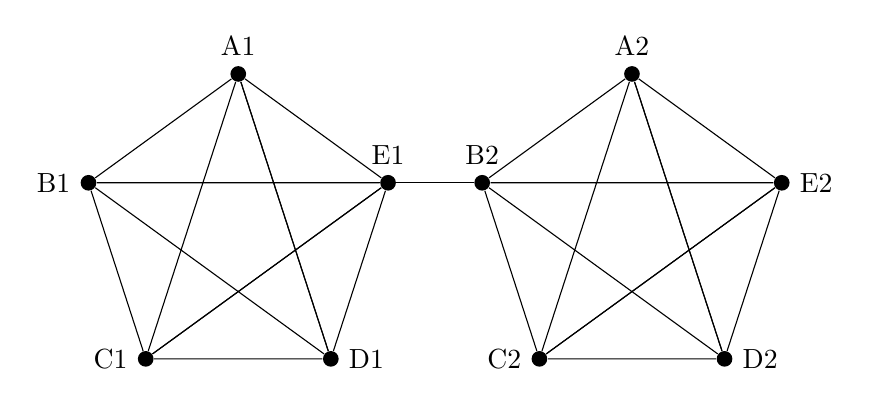
\begin{tikzpicture}
            % First K_5
            \begin{scope}[shift={(0,0)}]
                \node[circle, fill=black, inner sep=2pt, label=above:A1] (A1) at (90:2) {};
                \node[circle, fill=black, inner sep=2pt, label=left:B1] (B1) at (162:2) {};
                \node[circle, fill=black, inner sep=2pt, label=left:C1] (C1) at (234:2) {};
                \node[circle, fill=black, inner sep=2pt, label=right:D1] (D1) at (306:2) {};
                \node[circle, fill=black, inner sep=2pt, label=above:E1] (E1) at (18:2) {};
                \draw (A1) -- (B1) -- (C1) -- (D1) -- (E1) -- (A1);
                \draw (A1) -- (C1) -- (E1) -- (B1) -- (D1) -- (A1);
                \draw (A1) -- (D1);
                \draw (B1) -- (E1);
                \draw (C1) -- (E1);
            \end{scope}

            % Second K_5
            \begin{scope}[shift={(5,0)}]
                \node[circle, fill=black, inner sep=2pt, label=above:A2] (A2) at (90:2) {};
                \node[circle, fill=black, inner sep=2pt, label=above:B2] (B2) at (162:2) {};
                \node[circle, fill=black, inner sep=2pt, label=left:C2] (C2) at (234:2) {};
                \node[circle, fill=black, inner sep=2pt, label=right:D2] (D2) at (306:2) {};
                \node[circle, fill=black, inner sep=2pt, label=right:E2] (E2) at (18:2) {};
                \draw (A2) -- (B2) -- (C2) -- (D2) -- (E2) -- (A2);
                \draw (A2) -- (C2) -- (E2) -- (B2) -- (D2) -- (A2);
                \draw (A2) -- (D2);
                \draw (B2) -- (E2);
                \draw (C2) -- (E2);
            \end{scope}

            % Connecting edge between the two K_5 graphs
            \draw (E1) -- (B2);
        \end{tikzpicture}
        \caption{Povezana grafa \(K_5\)}
    \end{figure}
    Dvem polnim grafom \(K_n\) dodamo povezavo, da dobimo povezan graf \(G = (V,E)\). Če za \(S\) vzamemo enega izmed polnih grafov, je \(\lvert S\rvert = n\) maksimalen in \(\lvert \partial S\rvert = 1\) minimalen. Torej je Cheegerjeva konstanta
    \begin{align*}
        c(G) = \frac{1}{n}.
    \end{align*}
    Večji kot je \(n\), bolj izrazito je ozko grlo na grafu, kar vidimo tudi v manjši \(c(G)\).
\end{primer}
\subsection{Spektralna vrzel}
\subsection{Cheegerjeva neenakost}
\subsection{Alon-Boppanov izrek}
\subsection{Ramanujanovi grafi}